\documentclass[10pt,journal,compsoc, twoside]{IEEEtran}

% multirows
\usepackage{multirow}

\usepackage{setspace}

\usepackage{subfigure}  

\usepackage{amsmath,amssymb,amsfonts}
\usepackage{textcomp}

\usepackage[linesnumbered, ruled, vlined]{algorithm2e}

\usepackage{booktabs}
\usepackage{tikz}

% chinese
%\usepackage[UTF8]{ctex}

\usepackage{listings}
\usepackage{xcolor}
\lstset{
	numbers=left, 
	numberstyle= \tiny\tiny, 
	keywordstyle= \color{ blue!70},
	commentstyle= \color{red!50!green!50!blue!50}, 
	frame=shadowbox, 
	rulesepcolor= \color{ red!20!green!20!blue!20} ,
	escapeinside=``,
	xleftmargin=2em,xrightmargin=2em, aboveskip=1em,
	framexleftmargin=2em
} 


\renewcommand\labelenumi{(\roman{enumi})}
\renewcommand\theenumi\labelenumi

\makeatletter
\def\hlinew#1{%
	\noalign{\ifnum0=`}\fi\hrule \@height #1 \futurelet
	\reserved@a\@xhline}

%\usepackage{amsmath,amssymb,amsfonts}
% caption
%\usepackage{caption}
%\DeclareCaptionLabelSeparator{emdash}{\textemdash}
%\captionsetup[figure]{labelsep=emdash,font=onehalfspacing,position=bottom}
%\captionsetup{%
%	singlelinecheck=off,
%	skip=2pt,
%	justification=centering,
%}


% *** CITATION PACKAGES ***
%
\ifCLASSOPTIONcompsoc
  % The IEEE Computer Society needs nocompress option
  % requires cite.sty v4.0 or later (November 2003)
  \usepackage[nocompress]{cite}
\else
  % normal IEEE
  \usepackage{cite}
\fi


% *** GRAPHICS RELATED PACKAGES ***
%\usepackage[pdftex]{graphicx}
%
%\ifCLASSINFOpdf
%   \usepackage[pdftex]{graphicx}
%  % declare the path(s) where your graphic files are
%  % \graphicspath{{../pdf/}{../jpeg/}}
%  % and their extensions so you won't have to specify these with
%  % every instance of \includegraphics
%  % \DeclareGraphicsExtensions{.pdf,.jpeg,.png}
%\else
%  % or other class option (dvipsone, dvipdf, if not using dvips). graphicx
%  % will default to the driver specified in the system graphics.cfg if no
%  % driver is specified.
%   \usepackage[dvips]{graphicx}
%  % declare the path(s) where your graphic files are
%  % \graphicspath{{../eps/}}
%  % and their extensions so you won't have to specify these with
%  % every instance of \includegraphics
%  % \DeclareGraphicsExtensions{.eps}
%\fi


% NOTE: PDF hyperlink and bookmark features are not required in IEEE
%       papers and their use requires extra complexity and work.
% *** IF USING HYPERREF BE SURE AND CHANGE THE EXAMPLE PDF ***
% *** TITLE/SUBJECT/AUTHOR/KEYWORDS INFO BELOW!!           ***
\newcommand\MYhyperrefoptions{bookmarks=true,bookmarksnumbered=true,
pdfpagemode={UseOutlines},plainpages=false,pdfpagelabels=true,
colorlinks=true,linkcolor={black},citecolor={black},urlcolor={black},
pdftitle={Bare Demo of IEEEtran.cls for Computer Society Journals},%<!CHANGE!
pdfsubject={Typesetting},%<!CHANGE!
pdfauthor={Michael D. Shell},%<!CHANGE!
pdfkeywords={Computer Society, IEEEtran, journal, LaTeX, paper,
             template}}%<^!CHANGE!

% correct bad hyphenation here
\hyphenation{op-tical net-works semi-conduc-tor}



\begin{document}



\title{Measurements, Analysis and Modeling of Hyperledger Fabric}



%: Design, Implementation and Evaluation
%
%towards bandwidth and storage efficient blockchain on hyperledger


%\title{Towards Efficient Blockchain Storage on Hyperledger Fabric: Design, Implementation and Evaluation}

%\title{Towards Storage and Bandwidth Efficient Blockchain over Hyperledger Fabric: Design, Implementation, and Evaluation}
	
%	Hyperledger-Erasure: Towards A Storage and Bandwidth Efficient Blockchain System}

%\title{Storage and Bandwidth Efficient Blockchain Storage for }

%\title{Measurement and Analysis of the Bitcoin\\ Networks: A View from Mining Pools}


%\author{Canhui~Wang,~\IEEEmembership{Graduate Student Member,~IEEE,}
%        Xiaowen~Chu,~\IEEEmembership{Senior Member,~IEEE,}
%        and~Qin~Yang,~\IEEEmembership{Senior~Member,~IEEE}% <-this % stops a space
%        
%\IEEEcompsocitemizethanks{
%	
%	\IEEEcompsocthanksitem C. Wang is with Department of Computer Science, Hong Kong Baptist University, Kowloon Tong, Kowloon, Hong Kong, China. E-mail: chwang@comp.hkbu.edu.hk.
%
%	\IEEEcompsocthanksitem X. Chu is with Department of Computer Science, Hong Kong Baptist University, Kowloon Tong, Kowloon, Hong Kong, China. E-mail: chxw@comp.hkbu.edu.hk.
%
%	\IEEEcompsocthanksitem Q. Yang is with Department of Computer Science and Technology, Harbin Institute of Technology Shenzhen Graduate School, Shenzhen, China. E-mail: csyqin@hitsz.edu.cn.}% <-this % stops a space
%
%\thanks{Manuscript received XX XX, XXXX. (Corresponding author: Xiaowen Chu.)}
%
%}

% The paper headers
%\markboth{IEEE TRANSACTIONS ON PARALLEL AND DISTRIBUTED SYSTEMS. ,~Vol.~XX, No.~X, XX~XXXX}
%{C.  Wang \MakeLowercase{\textit{et al.}}: Measurement and Analysis of Bitcoin Networks: A View from Mining Pools}


\IEEEtitleabstractindextext{%

\begin{abstract}
	
Bitcoin network

\end{abstract}


% Note that keywords are not normally used for peerreview papers.
\begin{IEEEkeywords}
Bitcoin Network, Mining Pools, Malthusian Trap, Incentive Mechanism
\end{IEEEkeywords}}


% make the title area
\maketitle
\IEEEdisplaynontitleabstractindextext
\IEEEpeerreviewmaketitle


\ifCLASSOPTIONcompsoc
\IEEEraisesectionheading{\section{Introduction}\label{sec:introduction}}
\else
\section{Introduction}
\label{sec:introduction}
\fi



\IEEEPARstart{B}{itcoin} \cite{nakamoto2008bitcoin} is a decentralized peer to peer (P2P) cryptocurrency that was first proposed by Satoshi Nakamoto in 2008. Without resorting to any trusted third party, Bitcoin adapts a cryptographic proof mechanism that enables anonymous peers to complete transactions through the P2P network. Blockchain is the core mechanism of the Bitcoin system. It not only records historical transactions from Bitcoin clients, but also prevents the Bitcoin network from double spending attacks \cite{karame2015misbehavior}. The Bitcoin network participants, who maintain and update the ongoing chain of blocks, are called miners. These miners compete in a mining race driven by an incentive mechanism \cite{lewenberg2015bitcoin, schrijvers2016incentive}, where the one who first solves the Bitcoin cryptographic puzzle \cite{giechaskiel2016bitcoin} has the right to collect unconfirmed transactions into a new block, append the new block to the main chain, i.e., the longest chain of blocks, and gain some BTCs \cite{BTC} as a mining reward.



\section{Preliminary}

\subsection{Cluster Configuration}

This is about cluster configuration



\subsection{MSP}

Certificates




\subsection{TLS}

TLS secure protocol descrition








\section{Environment}

Hyperledger Fabric version 1.4

Fabric SDK v1.0.0

Jmeter




\section{BlockTime Solo Orderer Mode}

\subsection{Model Definition}

\begin{table}[]
	\caption{Configuration Notations}
	\begin{tabular}{|l|l|}
		\hline
		Notations    & Descriptions                                                                                             \\ \hline
		$N_{msg}$    & MaxMessageCount                                                                                          \\ \hline
		$S_{max}$    & AbsoluteMaxBytes                                                                                         \\ \hline
		$S_{pref}$   & PreferredMaxBytes                                                                                        \\ \hline
		$T_{batch}$  & \begin{tabular}[c]{@{}l@{}}Time to generate a block when MaxMessageCount\\ is not satisfied\end{tabular} \\ \hline
	\end{tabular}
\end{table}




\begin{table}[]
	\caption{Customized Notations}
	\begin{tabular}{|l|l|}
		\hline
		Notations     & Descriptions                                                                                         \\ \hline
		$T_{\sigma}$  & \begin{tabular}[c]{@{}l@{}}Time to generate a block when MaxMessageCount\\ is satisfied\end{tabular} \\ \hline
		$TAR$         & Transaction arrival rate                                                                             \\ \hline
		$BlockTime$   & Time it takes to generate a block                                                                    \\ \hline
		$TxDelay$     & Time it takes to issue a transaction                                                                 \\ \hline
		$S_{payload}$ & Size of transaction payload                                                                          \\ \hline
		$Throughput$     & Throughput of transactions                                                                 \\ \hline
	\end{tabular}
\end{table}







\subsection{Model of Orderer's Configuration}

The configuration file, i.e., configtx.yaml, configures the orderer service as follows.

\begin{lstlisting}
BatchTimeout: 2s
BatchSize:
   MaxMessageCount: 10
   AbsoluteMaxBytes: 98 MB
   PreferredMaxBytes: 512 KB
\end{lstlisting}


Case Study 1 without considering block size, we have the following model, Given a $TAR$ of which $\Delta t=1$, the time it costs is given as follows, the average block time is,


\begin{equation}
	BlkTime=\left\{
	\begin{array}{rcl}
	\infty  & & {TAR=0}\\
	$$T_{batch}$$ & & $$0 < TAR \leq \frac{N_{msg}}{T_{batch}}$$\\
	\frac{N_{msg}}{TAR} && \frac{N_{msg}}{T_{batch}}<TAR\leq \frac{N_{msg}}{T_{\sigma}}\\
	$$\left \lfloor \frac{TAR}{N_{msg}}-1 \right \rfloor \cdot T_\sigma$$  & & $$\frac{N_{msg}}{T_{\sigma}}< TAR, TAR\mid N_{msg} $$\\
	\left \lfloor \frac{TAR}{N_{msg}}-1 \right \rfloor \cdot T_\sigma + T_{batch}  & & otherwise
	\end{array} \right.
\end{equation}

%\begin{equation}
%Time=\left\{
%\begin{array}{rcl}
%\infty  & & {TAR=0}\\
%$$T_{batch}$$ & & $$0 < Tar \leq \frac{N_{msg}}{T_{batch}}$$\\
%$$\left \lfloor \frac{TAR}{N_{msg}}-1 \right \rfloor \cdot T_\sigma$$  & & $$\frac{N_{msg}}{T_{batch}}< TAR, TAR\mid N_{msg} $$\\
%\left \lfloor \frac{TAR}{N_{msg}}-1 \right \rfloor \cdot T_\sigma + T_{batch}  & & otherwise
%\end{array} \right.
%\end{equation}

If $TAR=0$, then $BlockTime=\infty$. It means that if there are no transactions, there are no blocks.

If $0 < TAR \leq \frac{MaxMessageCount}{BatchTimeout}$. It means that the number of transactions are less than MaxMessageCount given a BatchTimeout. Therefore, blocks are created for each BatchTimeout.

If $\frac{MaxMessageCount}{BatchTimeout}< TAR$. It means that the number of transactions are larger than MaxMessageCount in each BatchTimeout. Therefore, blocks are created as soon as possible and $\sigma$ is a small value.



\begin{figure}[htbp]
	\centering
	\scalebox{.8}{
		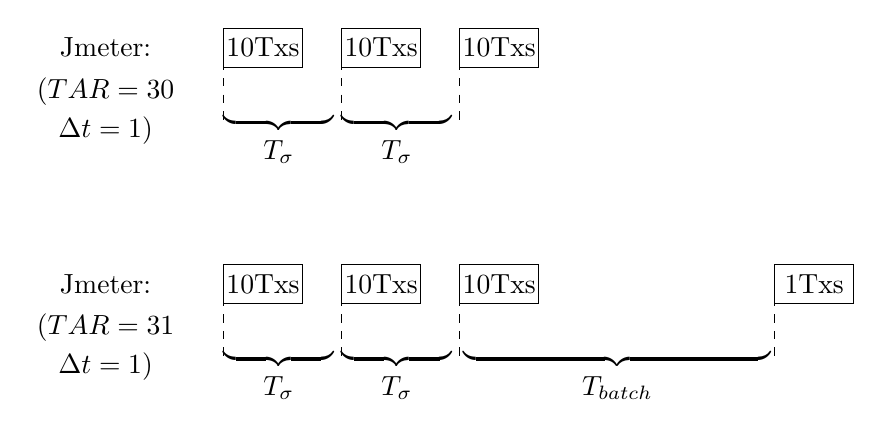
\begin{tikzpicture}
		
		% Jmeter
		\node [below] at (-2, 0+3) {Jmeter:};
		\node [below] at (-2, -0.5+3) {($TAR=30$};
		\node [below] at (-2, -1+3) {$\Delta t=1$)};
		
		% node 1
		\node [below] at (0, 0+3) {10Txs};
		\draw (-0.5,-0.5+3) rectangle (0.5,0+3);
		
		% node 2
		\node [below] at (0+1.5, 0+3) {10Txs};
		\draw (-0.5+1.5,-0.5+3) rectangle (0.5+1.5,0+3);
		
		% node 3
		\node [below] at (0+3, 0+3) {10Txs};
		\draw (-0.5+3,-0.5+3) rectangle (0.5+3,0+3);
		
		% node 4
		% \node [below] at (0+7, 0+3) {1Txs};
		% \draw (-0.5+7,-0.5+3) rectangle (0.5+7,0+3);
		
		% dash line of node 1
		\draw  [dashed](0-0.5,0+3) -- (0-0.5,-1.2+3);
		\node[rotate = 360] at (0.2, -1.2+3) {$\underbrace{\hspace{1.4cm}}$};
		\node [below] at (0.2, -1.3+3) {$T_{\sigma}$};
		
		% dash line of node 2
		\draw  [dashed](0-0.5+1.5,0+3) -- (0-0.5+1.5,-1.2+3);
		\node[rotate = 360] at (0.2+1.5, -1.2+3) {$\underbrace{\hspace{1.4cm}}$};
		\node [below] at (0.2+1.5, -1.3+3) {$T_{\sigma}$};
		
		% dash line of node 3
		\draw  [dashed](0-0.5+3,0+3) -- (0-0.5+3,-1.2+3);
		
		% dash line of node 3
		% \draw  [dashed](0-0.5+7,0+3) -- (0-0.5+7,-1.2+3);
		% \node[rotate = 360] at (4.5, -1.2+3) {$\underbrace{\hspace{3.9cm}}$};
		% \node [below] at (4.5, -1.3+3) {$T_{batch}$};
		
		
		
		% ------------------------------------------------------
		% Jmeter
		\node [below] at (-2, 0) {Jmeter:};
		\node [below] at (-2, -0.5) {($TAR=31$};
		\node [below] at (-2, -1) {$\Delta t=1$)};
		
		% node 1
		\node [below] at (0, 0) {10Txs};
		\draw (-0.5,-0.5) rectangle (0.5,0);
		
		% node 2
		\node [below] at (0+1.5, 0) {10Txs};
		\draw (-0.5+1.5,-0.5) rectangle (0.5+1.5,0);
		
		% node 3
		\node [below] at (0+3, 0) {10Txs};
		\draw (-0.5+3,-0.5) rectangle (0.5+3,0);
		
		% node 4
		\node [below] at (0+7, 0) {1Txs};
		\draw (-0.5+7,-0.5) rectangle (0.5+7,0);
		
		% dash line of node 1
		\draw  [dashed](0-0.5,0) -- (0-0.5,-1.2);
		\node[rotate = 360] at (0.2, -1.2) {$\underbrace{\hspace{1.4cm}}$};
		\node [below] at (0.2, -1.3) {$T_{\sigma}$};
		
		% dash line of node 2
		\draw  [dashed](0-0.5+1.5,0) -- (0-0.5+1.5,-1.2);
		\node[rotate = 360] at (0.2+1.5, -1.2) {$\underbrace{\hspace{1.4cm}}$};
		\node [below] at (0.2+1.5, -1.3) {$T_{\sigma}$};
		
		% dash line of node 3
		\draw  [dashed](0-0.5+3,0) -- (0-0.5+3,-1.2);
		
		% dash line of node 3
		\draw  [dashed](0-0.5+7,0) -- (0-0.5+7,-1.2);
		\node[rotate = 360] at (4.5, -1.2) {$\underbrace{\hspace{3.9cm}}$};
		\node [below] at (4.5, -1.3) {$T_{batch}$};
		
		\end{tikzpicture}
		
	}
	\caption{The $TAR$ Configurations}
\end{figure}




\subsubsection{Experiment 1: How $TAR$ affects $T_{sigma}$ and Throughput}

In this section, we focus on how $TAR$ affects the block time when MaxMessageCount is satisfied.

% Please add the following required packages to your document preamble:
% \usepackage[normalem]{ulem}
% \useunder{\uline}{\ul}{}
\begin{table*}[htbp]
	\caption{Experiment 1: $TAR$ affects $T_{sigma}$, $number of transactions of a block$ and $number of transactions rejected$}
	\begin{tabular}{|l|l|l|l|l|l|l|l|l|l|l|}
		\hline
		$TAR$           & 20    & 30     & 40     & 50     & 60     & 70     & 80              & 90              & 100             & \underline{150 }      \\ \hline
		$BlkTime$.AVG & 0.338 & 0.3828 & 0.4151 & 0.4035 & 0.5730 & 0.4866 & \textbf{1.1803} & \textbf{1.1792} & \textbf{1.0968} & \textbf{1.0285} \\ \hline
		$BlkTime$.MAX & 0.325 & 0.4040 & 0.5727 & 0.5260 & 0.6412 & 0.5290 & \textbf{1.5029} & \textbf{1.5668} & \textbf{1.3033} & \textbf{1.4904} \\ \hline
		$BlkTime$.MIN & 0.35  & 0.3715 & 0.3337 & 0.3362 & 0.4634 & 0.4492 & 0.6994          & 0.4832          & 0.7277          & 0.7244          \\ \hline
	\end{tabular}
\end{table*}

Experiment 1 -- Setup: for normal TAR we can use workload generators "Thread Group" on Ubuntu 01; while for small TAR we can use other workload generators "Ultimate Thread Group" on Ubuntu 01.

Experiment 1 -- Setup: for experiment analysis, we can check with logs in a peer. We have a program to analyze the log data, see $readdata.py$ at Github benchmark module at the $q3 v1 4$ folder.  


Experiment 1 -- Observation 1: when TAR achieves a high value (e.g., 80 tps, 90 tps), then a block cannot be fully make used (e.g., 8 transactions per block + 2 transactions per block, instead of 10 transactions per block).

Experiment 1 -- Observation 2: when TAR achieve a very high value (e.g., 200 tps), then a peer cannot handle such a high frequent event, and the SDK client will be rejected by the peer. See more error about TAR=200 per peer, Error "peer0.org2.example.com:7051, PKIid:6830efc127d4818973edd435ee7df6fa6fdf3e23286479b1e34d1229266559b5 isn't responsive: EOF". -- To solve this problem, we need more distributed machines.

TO DO -- why 70 tps to 80 tps, much not-full used blocks are created?


% Please add the following required packages to your document preamble:
% \usepackage[normalem]{ulem}
% \useunder{\uline}{\ul}{}
\begin{table*}[htbp]
	\caption{Experiment 2: how batch of $TAR$ affects $T_{sigma}$}
	\begin{tabular}{|l|l|l|l|l|l|l|l|l|l|l|}
		\hline
		$TAR$           & 11     & 21     & 31     & 41     & 51     & 61     & 71     & 81              & 91              & {\underline{141}}    \\ \hline
		$BlkTime$.AVG & 2.2673 & 1.2507 & 1.0408 & 0.9152 & 0.7564 & 0.7073 & 0.7243 & \textbf{0.9656} & \textbf{0.7010} & \textbf{nll} \\ \hline
		$BlkTime$.MAX & 2.4900 & 1.2920 & 1.3040 & 1.1757 & 0.8044 & 0.8395 & 0.9021 & \textbf{1.3219} & \textbf{0.8963} & \textbf{nll} \\ \hline
		$BlkTime$.MIN & 2.0030 & 1.1800 & 0.8203 & 0.7715 & 0.7222 & 0.6288 & 0.5626 & 0.5490          & 0.5187          & nll          \\ \hline
	\end{tabular}
\end{table*}


Experiment 2 -- Observation 1: for small TAR (e.g., 20 tps, 30 tps, 40 tps, 60 tps), setting of $TAR$ (e.g., 11 tps, 21 tps, 31 tps, 51 tps) highly affect the $T_{sigma}$.

TODO --: for large TAR(e.g., 80 tps, 90 tps, 140 tps), why experiment 2 is much lower than experiement 1?

TO DO --: why $TAR$=91 results in fewer null-fully used blocks than $TAR$=90? 





\subsubsection{Endorsement Policy (OR) on Transaction Delay}

Experiment 3 - Setup: Endorsement Policy (OR) the source code is at Ubuntu 01 - nodeTest invoke3.js.

Experiment 3 - Setup: we can calculate with timestamps at invoke3.js.

Experiment 3 - Setup: we save the timestamp results with Jmeter in a res.xml file.

Experiment 3 - Setup: we can summary the timestamp results with readxml.py at nodeTest in ubuntutu 01.

Experiment 3 - Setup: get proposal approval from localhost, see invoke3.js nodeTest in ubuntu 01.

Experiment 3: Set up: transaction payload size 2 bytes


\begin{table*}[htbp]
	\caption{Experiment 3: Endorsement Policy "OR", with local proposer}
	\begin{tabular}{|l|l|l|l|l|l|l|l|l|}
		\hline
		\multirow{2}{*}{$TAR$} & \multicolumn{2}{l|}{Phase 1: Tx Proposal Delay} & \multicolumn{2}{l|}{Phase 2: Tx Orderer Delay} & \multirow{2}{*}{Total Tx Delay} & \multirow{2}{*}{Rounds} & \multirow{2}{*}{Accepted Txs} & \multirow{2}{*}{Rejected Txs} \\ \cline{2-5}
		& Delay (s)              & Proportion (\%)        & Delay (s)             & Proportion (\%)        &                                 &                         &                               &                               \\ \hline
		5                      & 0.75                   & 24.67                  & 2.29                  & 75.33                  & 3.04                            & 5                       & 25                            & 0                             \\ \hline
		10                     & 1.52                   & 71.69                  & 0.60                  & 28.31                  & 2.12                            & 5                       & 50                            & 0                             \\ \hline
		30                     & 4.58                   & 82.67                  & 0.96                  & 17.33                  & 5.54                            & 5                       & 150                           & 0                             \\ \hline
		50                     & 7.88                   & 85.65                  & 1.32                  & 14.35                  & 9.2                             & 5                       & 250                           & 0                             \\ \hline
		70                     & 11.19                  & 88.11                  & 1.51                  & 11.89                  & 12.70                           & 5                       & 350                           & 0                             \\ \hline
		\textbf{90}            & \textbf{14.39}         & \textbf{89.10}         & \textbf{1.76}         & \textbf{10.90}         & \textbf{16.15}                  & \textbf{5}              & \textbf{436}                  & \textbf{14}                   \\ \hline
	\end{tabular}
\end{table*}


Experiment 3 - Observation 1: when $TAR$ are higher than 10 transactions per second, the transaction delay will increase up, since the length of the waiting line is longer.

Experiment 3 - Observation 2: when Tx Orderer Delay are larger than 3 seconds, the transaction proposal will be rejected.

Experiment 3 - Observation 3: transaction proposal delay increases linearly with transaction arrival rate, while orderer transaction delay is not.


Experiment 3 - Observation 4: why these 14 transactions are rejected? It is nothing about orderer. It is limited to the capacility of ubuntu01 local peer. While the next experiment 4, the ubuntu00 remote peer has more powerful computing capacity.

Optimal Solution to this problem: try to let different peers to help to send transaction proposals at the same time. 



\subsubsection{Endorsement Policy (OR) on Transaction Delay}

Experiment 4 - Setup: Endorsement Policy (OR) the source code is at Ubuntu 01 - nodeTest invoke3a.js.

Experiment 4 - Setup: we can calculate with timestamps at invoke3a.js.

Experiment 4 - Setup: we save the timestamp results with Jmeter in a res.xml file.

Experiment 4 - Setup: we can summary the timestamp results with readxml.py at nodeTest in ubuntutu 01.

Experiment 4: Set up: get proposal approval from remote peer, see invoke3a.js nodeTest in ubuntu 01.

Experiment 4: Set up: transaction payload size 2 bytes


\begin{table*}[htbp]
	\caption{Experiment 4: Endorsement Policy "OR", with remote proposer}
	\begin{tabular}{|l|l|l|l|l|l|l|l|l|}
		\hline
		\multirow{2}{*}{$TAR$} & \multicolumn{2}{l|}{Phase 1: Tx Proposal Delay} & \multicolumn{2}{l|}{Phase 2: Tx Orderer Delay} & \multirow{2}{*}{Total Tx Delay} & \multirow{2}{*}{Rounds} & \multirow{2}{*}{Accepted Txs} & \multirow{2}{*}{Rejected Txs} \\ \cline{2-5}
		& Delay (s)           & Proportion (\%)           & Delay (s)           & Proportion (\%)          &                                 &                         &                               &                               \\ \hline
		5                      & 0.80                & 26.05                     & 2.27                & 73.95                    & 3.07                            & 5                       & 25                            & 0                             \\ \hline
		10                     & 1.52                & 73.07                     & 0.56                & 26.93                    & 2.08                            & 5                       & 50                            & 0                             \\ \hline
		30                     & 4.51                & 83.82                     & 0.87                & 16.18                    & 5.38                            & 5                       & 150                           & 0                             \\ \hline
		50                     & 7.60                & 86.75                     & 1.16                & 13.25                    & 8.76                            & 5                       & 250                           & 0                             \\ \hline
		70                     & 10.88               & 88.62                     & 1.41                & 11.48                    & 12.29                           & 5                       & 350                           & 0                             \\ \hline
		90                     & 14.33               & 89.67                     & 1.65                & 10.33                    & 15.98                           & 5                       & 450                           & 0                             \\ \hline
	\end{tabular}
\end{table*}


Experiment 4 - Observation 1: we can not find any performance difference between local proposers and remote proposers.










\subsubsection{Endorsement Policy (AND) on Transaction Delay}

Experiment 5 - Setup: Endorsement Policy (AND) see Github benchmark module the config7.md and the config8.md files.

Experiment 5 - Setup: Endorsement Policy (AND) see invoke5.js at nodeTest folder in Ubuntu01 machine.


\begin{table*}[htbp]
	\caption{Experiment 5: Endorsement Policy "AND", with remote proposer}
	\begin{tabular}{|l|l|l|l|l|l|l|l|l|}
		\hline
		\multirow{2}{*}{$TAR$} & \multicolumn{2}{l|}{Phase 1: Tx Proposal Delay} & \multicolumn{2}{l|}{Phase 2: Tx Orderer Delay} & \multirow{2}{*}{Total Tx Delay} & \multirow{2}{*}{Rounds} & \multirow{2}{*}{Accepted Txs} & \multirow{2}{*}{Rejected Txs} \\ \cline{2-5}
		& Delay (s)           & Proportion (\%)           & Delay (s)           & Proportion (\%)          &                                 &                         &                               &                               \\ \hline
		5                      & 0.74                & 24.74                     & 2.25                & 75.25                    & 2.99                            & 5                       & 25                            & 0                             \\ \hline
		10                     & 1.56                & 71.88                     & 0.61                & 28.12                    & 2.17                            & 5                       & 50                            & 0                             \\ \hline
		30                     & 4.65                & 82.88                     & 0.96                & 17.12                    & 5.61                            & 5                       & 150                           & 0                             \\ \hline
		50                     & 7.82                & 86.12                     & 1.26                & 13.88                    & 9.08                            & 5                       & 250                           & 0                             \\ \hline
		70                     & 11.09               & 87.59                     & 1.57                & 12.41                    & 12.66                           & 5                       & 347                           & 3                             \\ \hline
		90                     & 14.34               & 88.62                     & 1.84                & 11.37                    & 16.18                           & 5                       & 438                           & 12                            \\ \hline
	\end{tabular}
\end{table*}



Experiment 5 - Observation 1: endorsement policy (AND) will have relatively small larger in transaction delay than endorsement policy (OR), when there are only two peers.

Experiment 5 - Observation 2: if the endorsement policy (AND), we will have more responses say two times, and the peer ubuntu00 will have double burdens, resulting in peer channel problem.

Experiment 5 - Next Steps: if we have more peers say 16 peers using the endorsement policy (AND), then how about the transaction delay?

Experiment 5: Next Steps: what is the technical solutions to the error problem with the eventhub? the eventhub shutdown problem see $https://stackoverflow.com/questions/52773529/hyperledger-fabric-nodejs-sdk-eventhub-has-been-shutdown$. Then try to build up your own queue on the peer nodes.

Solutions to the eventhub problem: build up your own queue $https://stackoverflow.com/questions/52773529/hyperledger-fabric-nodejs-sdk-eventhub-has-been-shutdown$. See Event hub with read-write conflict transactions $https://ieeexplore.ieee.org/stamp/stamp.jsp?arnumber=8751453$. 







\subsubsection{Transaction Size on Transaction Delay}

Experiment 6 - Setup: Transaction size 1 KB

Experiment 6 - Setup: invoke3.js in "nodeTest" folder in ubuntu 01.

\begin{table*}[htbp]
	\caption{Experiment 6: Transaction Size on Transaction Delay 1 KB}
	\begin{tabular}{|l|l|l|l|l|l|l|}
		\hline
		$TAR$ & Phase 1: Tx Proposal Delay & Phase 2: Tx Orderer Delay & Total Tx Delay & Rounds & Accepted Txs & Rejected Txs \\ \hline
		5     & 0.78                       & 2.33                      & 3.11           & 5      & 25           & 0            \\ \hline
		10    & 1.54                       & 0.68                      & 2.22           & 5      & 50           & 0            \\ \hline
		30    & 4.67                       & 0.94                      & 5.61           & 5      & 150          & 0            \\ \hline
		50    & 7.83                       & 1.25                      & 9.08           & 5      & 250          & 0            \\ \hline
		70    & 11.14                      & 1.48                      & 12.62          & 5      & 350          & 0            \\ \hline
		90    & 14.54                      & 1.86                      & 16.4           & 5      & 449          & 1            \\ \hline
	\end{tabular}
\end{table*}












\subsubsection{Transaction Size on Transaction Delay}

Experiment 7 - Setup: Transaction size 10 KB

Experiment 7 - Setup: invoke3.js in "nodeTest" folder in ubuntu 01.


























%\subsubsection{Experiment : linear and Uniform Random Distribution of TAR}
%
%Delay Definition: one request (thread) waits for some time, until next request is generated. We call this time "Delay", denoted by $Delay$.
%
%
%Model Definition: For a request i,  $Delay_i$ follows a uniform distribution between zero and $T$ seconds, as follows, Probability density function is as follows,
%
%\begin{equation}
%	f(Delay_i)=\left\{
%	\begin{array}{rcl}
%	0  & & {Delay_i< 0}\\
%	$$\frac{1}{T}$$ & & $$ 0 \leq  Delay_i \leq T$$\\
%	0  & & $$ T < Delay_i $$
%	\end{array} \right.
%\end{equation}











%\begin{table}[htbp]
%	\caption{Different Configuration of BatchTimeout}
%	\begin{tabular}{|l|l|l|l|l|l|l|l|}
%		\hline
%		BatchTimeout (s) & 0.1 & 0.5 & 1 & 2 & 5 & 10 & 30 \\ \hline
%		BlockTime (s)    & a   & a   & a & a & a & a  & a  \\ \hline
%	\end{tabular}
%\end{table}
%
%See experiment 1 and experiment 2
%
%Table shows how different configuration of BatchTimeout affect BlockTime. Following our model, and the experiments, we can have a comparison results as follows. Here we need a figure with a comparison of the model result and the experimental results.
%
%See more about Uniform Random Timer $http://2min2code.com/articles/jmeter_intro/random_timer$
%
%linear and uniform random distribution of TAR: $https://flood.io/blog/planning-for-high-concurrency-load-tests-with-jmeter/$ 





%\subsubsection{Experiment : Poisson Distribution of TAR}
%
%\begin{table}[htbp]
%	\caption{Different Configuration of BatchTimeout}
%	\begin{tabular}{|l|l|l|l|l|l|l|l|}
%		\hline
%		BatchTimeout (s) & 0.1 & 0.5 & 1 & 2 & 5 & 10 & 30 \\ \hline
%		BlockTime (s)    & a   & a   & a & a & a & a  & a  \\ \hline
%	\end{tabular}
%\end{table}
%
%Table shows how different configuration of BatchTimeout affect BlockTime. Following our model, and the experiments, we can have a comparison results as follows,
%
%Jmeter Poisson Distribution of TAR: $https://www.blazemeter.com/blog/comprehensive-guide-using-jmeter-timers/$
%
%Jmeter Poisson Distribution of TAR: $https://medium.com/@malith.jayasinghe/performance-testing-with-a-think-time-64b6b737e3f9$
%
%The lambda in the Poisson distribution is the average time between the completion of one request and the start of the next request.






%\subsubsection{Experiment : Constant Distribution of TAR}
%
%Jmeter Constant Distribution of TAR: $https://www.blazemeter.com/blog/comprehensive-guide-using-jmeter-timers/$
%
%\begin{table}[htbp]
%	\caption{Different Configuration of BatchTimeout}
%	\begin{tabular}{|l|l|l|l|l|l|l|l|}
%		\hline
%		BatchTimeout (s) & 0.1 & 0.5 & 1 & 2 & 5 & 10 & 30 \\ \hline
%		BlockTime (s)    & a   & a   & a & a & a & a  & a  \\ \hline
%	\end{tabular}
%\end{table}
%
%Table shows how different configuration of BatchTimeout affect BlockTime. Following our model, and the experiments, we can have a comparison results as follows,





\subsection{Transaction Delay (For Peer)}
 
Here we need to discuss something about transaction delay in this section. 


\subsubsection{Transaction Size}

How transaction size affects transaction delay, transaction loss

\subsubsection{Experiment 1: Transaction Size 1 byte}



\subsubsection{Experiment 2: Transaction Size 300 byte}



\subsubsection{Experiment 3: Transaction Size 10 Mbyte}








\subsubsection{Endorsement Policy} 

\subsubsection{Experiment 1: Policy a}


\subsubsection{Experiment 2: Policy b}


\subsubsection{Experiment 3: Policy c}

Here we need to know how endorsement policy affect transaction delay





\section{Kafka Orderer Mode}


\subsection{Model of Kafka Orderer's Configuration}

The configuration file of Kafka




% Can use something like this to put references on a page
% by themselves when using endfloat and the captionsoff option.
\ifCLASSOPTIONcaptionsoff
  \newpage
\fi


\bibliographystyle{IEEEtran}
\bibliography{tpds}

\vspace{240pt}




\end{document}


